\documentclass[a4paper,twoside]{article}

  \usepackage{verbatim}
   \usepackage{flushend}
\usepackage{epsfig}
\usepackage{subfigure}
\usepackage{calc}
\usepackage{amssymb}
\usepackage{amstext}
\usepackage{amsmath}
\usepackage{amsthm}
\usepackage{multicol}
\usepackage{pslatex}
\usepackage{apalike}
\usepackage{SciTePress}
\usepackage[small]{caption}

\subfigtopskip=0pt
\subfigcapskip=0pt
\subfigbottomskip=0pt

\begin{document}

\title{EEG Data Processor  \subtitle{Framework for Running Signal Processing Methods} }

\author{\authorname{Petr Je\v{z}ek\sup{1}, Roman Mou\v{c}ek\sup{2}}
\affiliation{\sup{1}New Technologies for the Information Society, \sup{2}Department of Computer Science and Engineering}
\affiliation{University of West Bohemia,}
\affiliation{Univerzitni 8, 306 14,}
\affiliation{Pilsen, Czech Republic}
\email{jezekp@ntis.zcu.cz, moucek@kiv.zcu.cz}
}

\keywords{EEG/ERP, Signal Processing, Data Processing, Plug-in, Methods, Discrete Wavelet Transform,  Complete Wavelet Transform, Matching Pursuit, Fast Independent Component Analysis, Finite Input Response, Fast Fourier Transform, Workflow, Software as Service}

\abstract{This paper introduces difficulties related with the EEG/ERP signal processing. Although several systems that implement signal processing methods exist their sharing and remote calling is not satisfactorily solved. Authors' present a custom server-side approach that provides a powerful plug-in engine for integration of signal processing methods. The plug-in engine ensures a high modularity and flexibility of the system. Because of implemented methods are accessible thought the SOAP Web Service integration with other system is available. System is also possible to use locally via a web browser. The set of basic methods is already implemented and presented. The architecture and the most important parts of the system are also presented.}

\onecolumn \maketitle \normalsize \vfill

\section{\uppercase{Introduction}}
\label{sec:introduction}

\noindent In our research group we specialize on research of brain activity. During our experiments we largely use methods of Electroencephalography (EEG) with ist subset Event-Related Potentials (ERP). Experiments are performed in specially equipped laboratory including recording devices, car simulator or soundproof room. When experiments are performed the experimental data/metadata has to be collected for future processing. Since neuroscience community is facing problems with the long-term storage of data/metadata, raw data analysis, data/metadata sharing or designing of experimental protocols the International Neuroinformatics Coordinating Facility (INCF)\footnote{http://www.incf.org/} released recommendations \cite{incf-sustainability-report} for the neurophysiological data dealing.

As the Czech National Node of INCF we cooperate on the definition of standardized data/metadata format for electrophysiology research. As an initial proposal we developed a central custom solution called the EEG/ERP Portal \cite{DBLP:conf/biostec/JezekM10}.

The EEG/ERP Portal is a web based system that enable users to store, share and manage custom experiments. The data are stored within the EEG/ERP Portal accessible through a web browser. In addition we provide data in the Semantic Web form available for automatic readers. The  Semantic Framework \cite{DBLP:conf/biostec/JezekM12} that we developed transforms data from the EEG/ERP Portal into the Semantic Web languages (OWL, RDF). The EEG/ERP Portal is registered within the Neuroscience Information Framework (NIF) \cite{DBLP:journals/ni/GardnerAABBDGGGGHKMMMMRSSEW08} it ensures easier searchability of stored experiments. The EEG/ERP Portal is also integrated with other developed systems (e. g. JERPA \cite{DBLP:conf/biostec/JezekM11}) via Web Service API.

Because of data from stored experiments are usually further processed using various signal processing methods we are presenting the EEG Data Processor that enables running of signal processing methods remotely.

\section{\label{sec:StateOfTheArt}\uppercase{State of the Art}}

\noindent When the data are collected they are supposed to be processed. The EEG/ERP Portal is supposed to store experimental data. When data are processed they need to be downloaded and processed locally. The obtained result are not stored as well. 

When we were looking for a suitable tool, we found that the set of available frameworks is limited. After investigating possibilities of existing tools we choose these that are able to process EEG/ERP experimental data.

The Carmen Portal \cite{fgibson:Watson2007} provides a set of implemented analytical tools. An user can upload a custom data into the local storage. The data can be analyzed and the results are putted into the virtual directory assigned to users' profiles. When the user wants to add a custom analytical tool he/she can upload it into the system. When this method is approved by Carmen administrators they will incorporate it into the system.

Carmen is only one well-known system that enables calling of analytical methods remotely together with the possibility to store experimental results.

The next approaches work locally without any possibilities to save or share experimental results.

Modular Toolkit for Data Processing (MDP) \cite{citeulike:3973843} is a data processing framework written in Python. MDP is a modular framework that can Python programmers extend by additional modules. Common users can call implemented modules locally.

BioSig \cite{BIOSIG} is a free open source software library of biomedical signal-processing tools implemented as a library for Matlab, Octave and C/C++. The last version of the tool called biosic4c++ can be also used in the Python. This system contains additional submodules for e.g. real-time data processing or a signal viewer.

Since a data processing often requires usage of more methods sequentially a creating of specific workflows is required.

Taverna \cite{citeulike:1041436} is an open source and domain-independent Workflow Management System developed by $^{my}Grid$\footnote{http://www.mygrid.org.uk/} team. It is a suite of tools used to design and execute scientific workflows and aid in silico experimentation.

E-Science Central \cite{Watson:2010:ECC:1873585.1873592} combines three emerging technologies Software as a Service, Social Networking and Cloud Computing.

The Carmen developers are also developing The CARMEN Workflow Tool. It is Java-based and designed to supports both data and control flow, and it allows parallel execution of services using a Service Invocation API

\section{\uppercase{EEG Data Processor}}

\subsection {\label{sec:Existing Approaches Difficulties}Existing Approaches Difficulties}

\noindent Although solutions described in Section \ref{sec:StateOfTheArt} work quite satisfactorily several difficulties stay. The most of tested tools work as stand-alone systems that a user has to install on a custom computer and run it on the data manually. The tools are implemented using various programming languages where each requires a specific runtime environment. It could be an obstacle for many users because it requires a certain level of user knowledge. The last disadvantages is an inability to integrate such systems with users solutions and control them from the custom client program.

\subsection{System Scope}

\noindent Because of difficulties mentioned in Subsection \ref{sec:Existing Approaches Difficulties} we have decided to implement a custom system that enables running of signal processing methods on data stored within the EEG/EEP Portal. The system is prepared to be integrated with the systems of other users or used independently.

The implemented methods are plug-ins based on Java platform. The libraries and whole system is provided as an open source. It ensures a higher availability for potential users and faster development of new plug-ins. Basically, the system is ligtweight wrapper for implemented plug-ins with double type user interface. First, is a standardized Web Service API, second one is an interactive web interface.

The focus of the EEG Data Processor is to be a software as a service (SaaS) delivery model. It offers reusing of software applications, the ability to compare processing algorithms and access to considerable computing resource for high intensity computing tasks.

\section{\uppercase{Design and Realization}}


\subsection{Architecture}

\noindent The system is a layered architecture. This architectural style is supported by used programming languages and technologies (Java, Maven, Spring, Hibernate, Apache CXF web services etc.)

  \begin{figure*}[t!]
	\centering
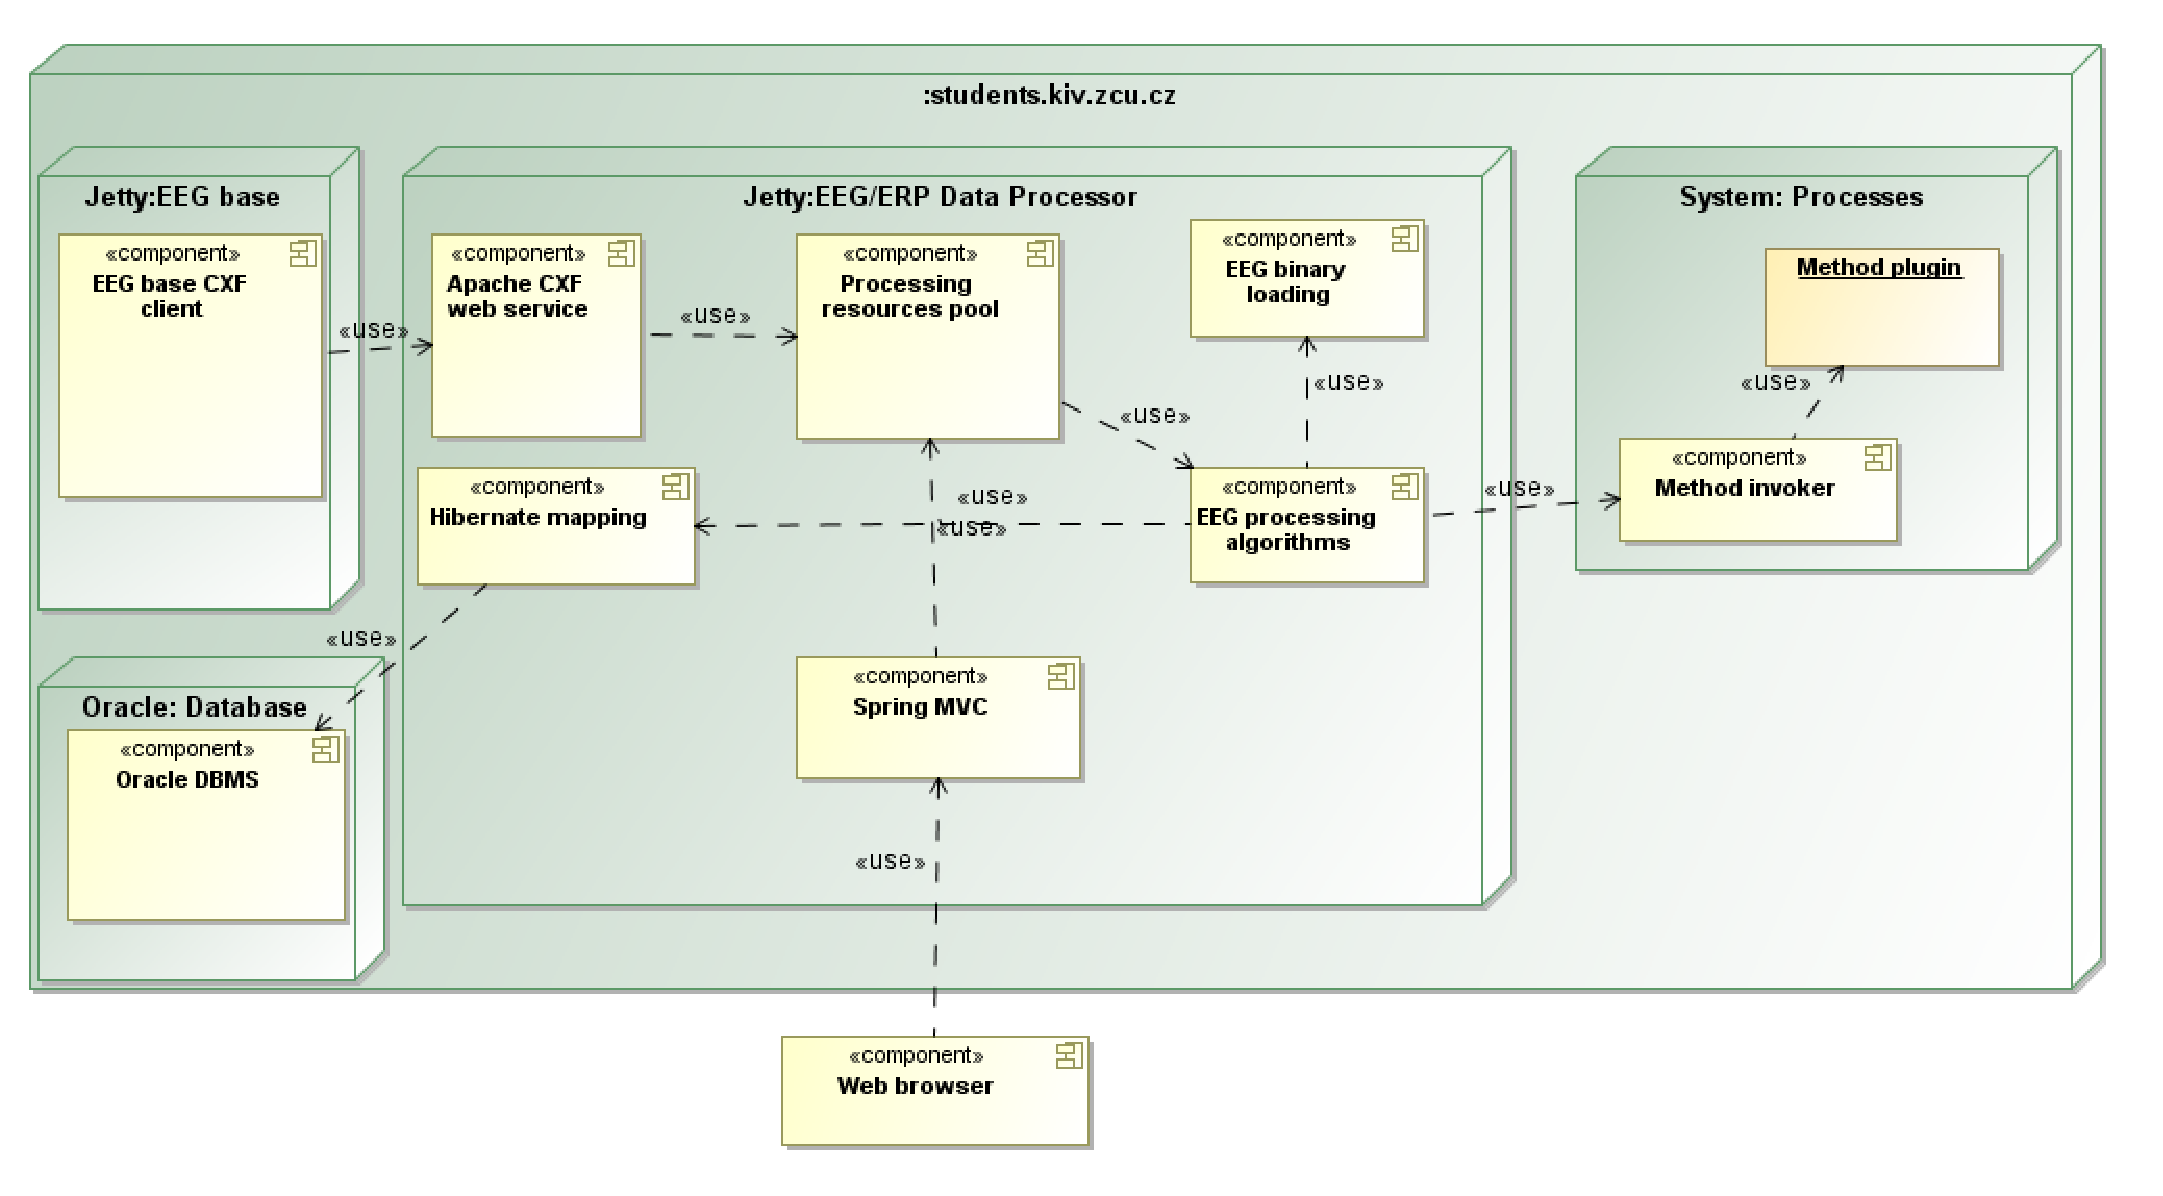
\includegraphics[width=14cm, height=8cm]{component_model}

\caption{\label{fig:component_model}Component Model}

\end{figure*}

The internal structure consists several components (see Figure. \ref{fig:component_model}). The main components of the system are:
\begin{itemize}
\item EEG Binary Loading - it loads data from binary files obtained from  an analogue-digital converter. We currently support the data obtained from the Brain Vision Recorder but the system is fully prepared for adding a support of a new data format without any difficulties.
    
\item Processing Resource Pool - Because of a performance capacity of the hosted server is limited we have implemented a pool of available resources. The system can be configured to manage a number of requests simultaneously. When this limit is reached other requirements are queued and gradually processed.
    
\item EEG Processing Algorithms - This module manages a running of installed plug-ins. It has access to list of installed plug-ins and calls a method invoker.

\item External Method Invoker - Its responsible for execution of the requested method. It fills the method parameters and takes the method result.
\end{itemize}

The significant modules of the system are described in following section.



\subsection{Significant Modules}

\subsubsection{\label{sec:Plug-in-Engine}Plug-in Engine}

\noindent A Plug-in engine is a central unit of the system. It contain an implementation of a Processor. The Processor is an abstraction of implemented EEG Binary Loading libraries that are intended to read input digitalized signal stored within various data formats. The Processor creates individual Processes. The Process is an encapsulation of a specific method together with the specific parameters needed to start the method.

When a new method is emerging it has to satisfy several conditions in order to be integrated into the system. First it should contain one input method with specified input parameters of the method and a XML description of the output. Because of output of  individual methods can be different (e.g waveforms, discrete points, etc.) the XML format ensures its easier future representation. Second, the method has to have an descriptive properties file that contains input name of the method, package and class. When the method is invoked by the described External Method Invoker it reads all parameters from the properties file and configures the created Process.


\subsubsection{Web Service Connector}

\noindent Since the EEG Data Processor is supposed to be accessed by external clients' systems the Web Service API best matches this requirement. The system provides a simple interface with a few basic methods. The client can obtain a list of installed methods, lists of required parameters for the specific method, get available processing units and call the method that processes input data. Such interface provide a sufficient list of operations in order to be integrated with any client system. A usage of SOAP web services ensures easy integration by a well-defined protocol.

\subsubsection{Web Interface}

\noindent Communication with users client system is ensured using Web Service Connector. In the case where user has only data but not a custom system connected to the Internet, we prepared a simple web based interface. Figure \ref{fig:system_overview} shows the interface overview. The user can list installed signal processing methods and available processing units. When he/she wants to upload a custom data a simple upload form is prepared. The uploaded data are stored within the user's profile and processed on the background. When the result is available a link to download appears.

  \begin{figure}[t!]
	\centering
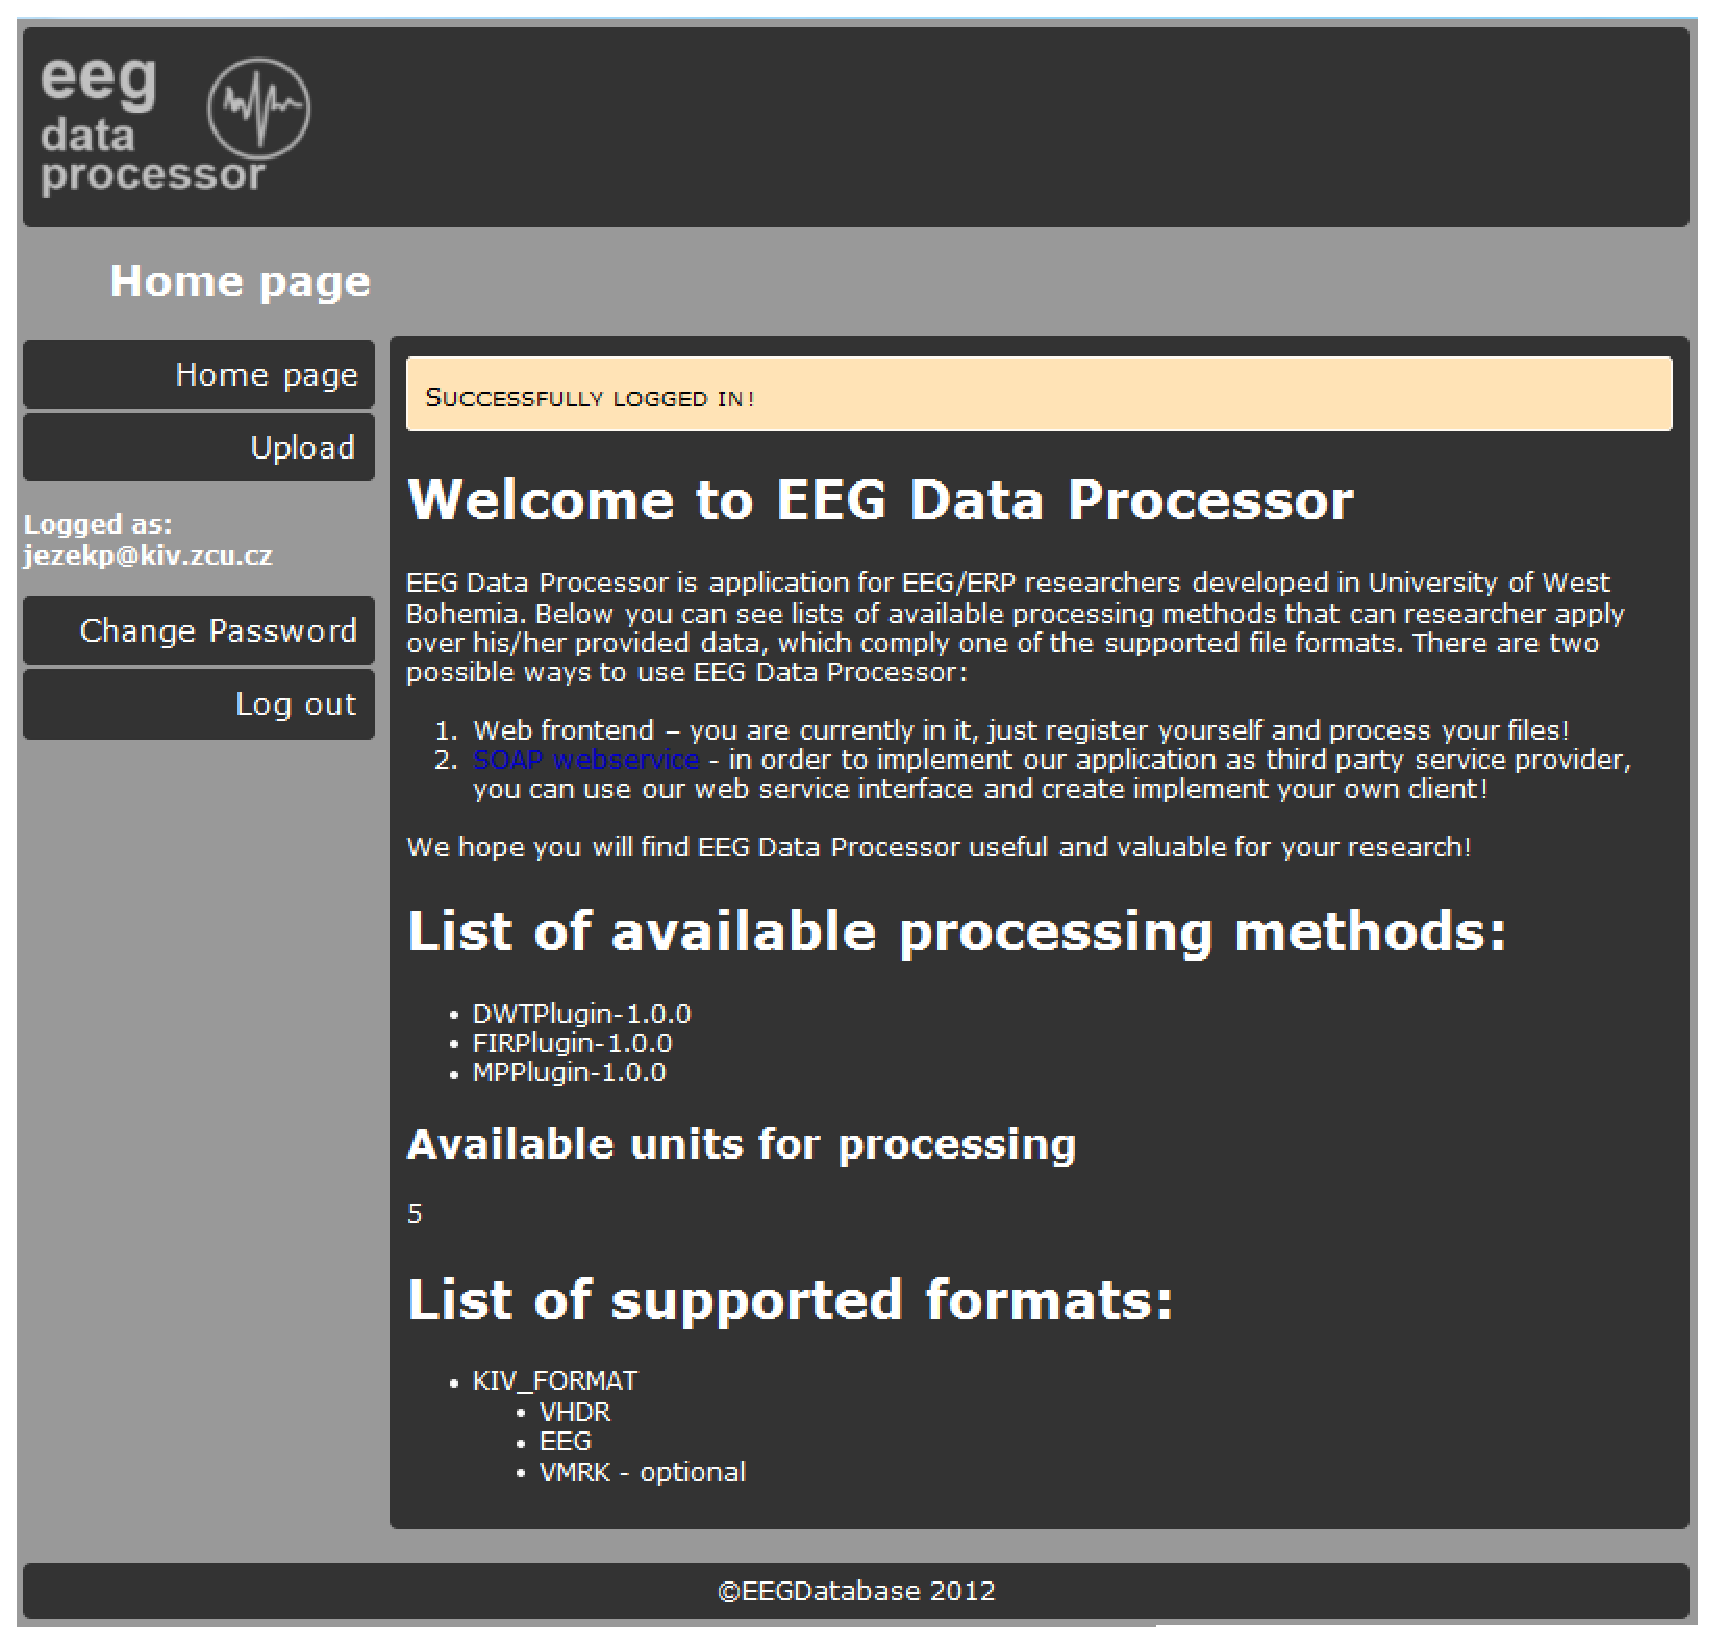
\includegraphics[width=7.5cm, height=7cm]{system_overview}

\caption{\label{fig:system_overview}Web Interface Overview}

\end{figure}

\subsection{System Security}

\noindent Since the system is public available through the Internet a secured access has to be ensured. The system is protected by system accounts with two possible user roles. The \emph{user} can upload a custom data that can be protected while the \emph{administrator} can manage registered users and configure the system. On the implementation level, the security is ensured by Spring Security framework with one way hashed user passwords with randomly generated salt.

The user can register into the system by filling simple registration form. When user accesses the system through the Web Services API the SSL transfer is ensured and users credentials are required.

\section{\uppercase{Implemented Plug-ins}}

\noindent We have already implemented methods that are most often used during experiments within our laboratory. Implemented methods are a common Java libraries extended according to the description in Section \ref{sec:Plug-in-Engine}. This architectural style ensures their implementation outside the system independently. Such libraries can be also put into any java-based system. Therefore, we provide implemented plug-ins open source putt in the public repositories (GitHub, SorceForge). The list of implemented methods is gradually expanding.

Currently, we have implemented following methods:

\begin{itemize}
\item
\textit{Complete and Discrete Wavelet Transform} \cite{DBLP:books/daglib/0098272} is a transform which localizes a function both in space and scaling and has some desirable properties compared to the Fourier transform. The transform is based on a wavelet matrix, which can be computed more quickly than the analogous Fourier matrix.

\item
\textit{Matching Pursuit} \cite{journals/toms/FerrandoKK02} decomposes any signal into a linear expansion of waveforms that are selected from a redundant dictionary of functions. These waveforms are chosen in order to best match the signal structure. The dictionary is often based on Gabor functions.

\item
\textit{Fast Independent Component Analysis} \cite{hyv�rinen2001independent} is used for finding a linear representation of nongaussian data so that the components are statistically independent, or as independent as possible. Such a representation seems to capture the essential structure of the data in many applications, including feature extraction and signal separation.

\item
\textit{Fast Fourier Transform} \cite{Fast-Fourier-Transform} is an efficient algorithm to compute the discrete Fourier transform (DFT) and its inverse. the discrete Fourier transform (DFT) is a specific kind of discrete transform, used in Fourier analysis. It transforms one function into another, which is called the frequency domain representation.

\item
\textit{Finite Input Response} is a digital filter that have an impulse response which reaches zero in a finite number of steps. It can be implemented non-recursively by convolving its impulse response.
\end{itemize}


\section{\uppercase{Current Status}}


\noindent The system is almost fully implemented and prepared for testing. We put in on the testing server where it is tested by the research group members. After that we enable the system for testing by the limited set of selected collaborative partners. When testing ends we released the system on the productional server.

\section{\uppercase{Future Work}}

\noindent When the system is released the next step will be an implementation of a client side within the EEG/ERP Portal. It allows to portal users a more comfortable work because the load will be distributed between two servers. Faster response will be ensured.

Since a need to associate methods into workflows was mentioned in Section \ref{sec:StateOfTheArt} we plan to implement a wokflow module into the system. This module will ensure a creation of custom workflows and stored them into users' accounts. We plan to make it easy to use by preparing an interface with drag and draw functionality.

The next research challenge leads in the sharing not only data and signal processing methods, but dissemination of knowledge about e. g. designing of experimental scenarios, results or data interpretation etc. Because of increasing popularity of social networks amount of provided information is rising. Such networks should be suitable medium for sharing information between researchers.

We plan to implement a custom internal social network in the system. The internal social network will be connected with external social networks (e. g. Facebook, Twitter or LinkedIn). When a user publish a comment to an internal social network it will be also possible to publish it on a selected external social network. In addition, a back synchronization is desirable. When a user is logged on external social network he/she can download comments into the internal social network. Our plan is to develop a framework that will automatically browse social networks and find comments according to defined rules.

Further, we plan to investigate possibilities in the area of Cloud Computing, because of a potential load of the server will increase in the raising number of users. The suitable cloud should help to improve a management of system resources. 

\section{\uppercase{Conclusions}}
\label{sec:conclusion}

\noindent The difficulties related with the processing of data from EEG/ERP experiments are presented. Because of implementation of present signal processing method is usually intended for local usage we decided to propose and implement a custom system. The aim of the presented system is to serve a wide researchers community to share experimental methods.

The system combines research in EEG/ERP with modern software engineering approaches. It helps to enhance research efficiency and enables a faster achieve of scientific results.

The most often used method in our laboratory are briefly presented. The presented method are already implemented and integrated within the system as plug-ins. Due to a powerful plug-in engine interested users are welcome to implement a custom method according to a described procedure. We are able to assume these plug-ins and incorporate them into the system.

Since the system is open-source developed using common open-source technologies the development of plug-ins is without difficulties.


\section*{\uppercase{Acknowledgements}}

\noindent It will be written in the camera ready paper.

%\vfill
\bibliographystyle{apalike}
{\small
\bibliography{bibliography}}


\vfill
\end{document}

